

\begin{figure}[t!]
\centering
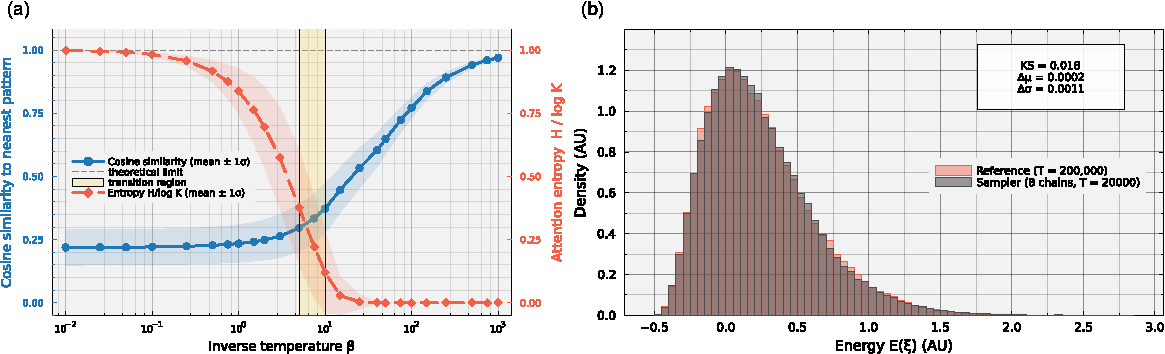
\includegraphics[width=\textwidth]{figs/Fig_experiment-combined.pdf}
\caption{Synthetic experiments.
\textbf{(a)}~Phase behavior as a function of inverse temperature $\beta$ ($d=64$, $K=16$). Left axis (blue): mean cosine similarity to the nearest stored pattern; right axis (coral): scaled entropy $H(\mathbf{a})/\log K$. Both diagnostics reveal a smooth transition centered near $\beta\approx 5\text{--}10$ (gold band).
\textbf{(b)}~Convergence validation ($d=8$, $K=4$, $\beta=5$). Pooled energy density from eight independent chains (gray) overlaid on a long-run reference distribution (coral); inset reports the Kolmogorov--Smirnov statistic and moment differences.}
\label{fig:experiments}
\end{figure}

\paragraph{Synthetic validation.}
We constructed memory matrices with columns drawn uniformly from $\mathbb{S}^{d-1}$ (the standard model in the Hopfield capacity literature~\cite{amitStoringInfiniteNumbers1985}). All experiments used step size $\alpha=0.01$ with fixed random seeds. We first evaluated how $\beta$ controlled the retrieval-to-generation transition (Fig.~\ref{fig:experiments}a): with $K=16$ patterns in $d=64$, both cosine similarity and attention entropy exhibited a smooth sigmoidal transition centered near $\beta\approx 5$--$10$, confirming that $\beta$ acted as a continuous order parameter analogous to the classical Hopfield/Boltzmann transition~\cite{ackleyLearningAlgorithmBoltzmann1985}. The variance of both diagnostics peaked in the transition region, where the chain intermittently switched between pattern-aligned and exploratory states. A convergence experiment on a small system ($d=8$, $K=4$, $\beta=5$; Fig.~\ref{fig:experiments}b) confirmed that eight independent chains converged to the correct Boltzmann target, with pooled energies matching a long-chain reference. A load-ratio phase diagram (Fig.~\ref{fig:phase-diagram}) over $K/d\in[0.05,2.0]$ and $\beta\in[0.5,100]$ revealed a clear phase boundary: retrieval at high $\beta$ and low $K/d$, with the boundary shifting rightward as $\beta$ increased, consistent with classical capacity theory.

% ---------- Experiment 4: MNIST Baseline Comparison ----------
\paragraph{Image generation on MNIST.}
We selected $K=100$ images of the digit ``3'' from MNIST~\cite{lecunGradientBasedLearningApplied1998}, flattened to $\mathbb{R}^{784}$ and $\ell_2$-normalized. Because the energy landscape at high $\beta$ is deeply multimodal, we launched 30 independent chains, each initialized near a different stored pattern ($\sigma_{\mathrm{init}}=0.01$), run at $\beta=2000$ with $\alpha=0.01$ for $T=5{,}000$ iterations (burn-in $2{,}000$, thinning every 100th step), retaining $150$ samples spanning 30 basins. The choice $\beta=2000$ follows from the SNR analysis: the per-step signal-to-noise ratio
\begin{equation}
\mathrm{SNR}
\;=\;\sqrt{\frac{\alpha\beta}{2d}}\,,
\label{eq:snr}
\end{equation}
undergoes a critical transition at $\mathrm{SNR}^{*}=\sqrt{\alpha/(2\sqrt{d})}$ (Eq.~\ref{eq:snr-star}). At $d{=}64$ and $\alpha{=}0.01$ this gives $\mathrm{SNR}^{*}=0.025$ ($\beta^{*}\approx 8$), consistent with the observed transition; we set $\beta=2000$ ($\mathrm{SNR}=0.113$) for structured retrieval.

We compared against seven baselines using the same memory matrix: bootstrap resampling, Gaussian perturbation ($\sigma=\sqrt{2\alpha/\beta}$), random convex combination ($\mathbf{w}\sim\mathrm{Dirichlet}(1,\dots,1)$), Gaussian mixture model with PCA preprocessing (GMM-PCA; 50 components, 10 clusters; Appendix~\ref{app:gmm-pca}), variational autoencoder (VAE; latent dim 8; Appendix~\ref{app:vae}), denoising diffusion probabilistic model (DDPM; MLP-based, $T{=}200$ steps; Appendix~\ref{app:ddpm}), and Metropolis-adjusted Langevin algorithm (MALA; same Langevin proposal with accept/reject correction). For each method we generated 150 samples and evaluated novelty~$\mathcal{N}$, diversity~$\bar{\mathcal{D}}$, and mean energy~$\bar{E}$:
\begin{align*}
\mathcal{N}(\hat{\boldsymbol{\xi}}) = 1 - \max_{k}\cos\!\bigl(\hat{\boldsymbol{\xi}},\,\mathbf{m}_{k}\bigr),\qquad
\bar{\mathcal{D}} = \frac{2}{S(S{-}1)}\!\sum_{i<j}\bigl(1-\cos(\hat{\boldsymbol{\xi}}_i,\hat{\boldsymbol{\xi}}_j)\bigr),\qquad
\bar{E} = \frac{1}{S}\sum_{i=1}^{S} E\!\bigl(\hat{\boldsymbol{\xi}}_i\bigr),
\end{align*}
where $\cos(\mathbf{x},\mathbf{y})=\mathbf{x}^{\top}\mathbf{y}/(\lVert\mathbf{x}\rVert\,\lVert\mathbf{y}\rVert)$. Novelty measures departure from stored patterns; diversity is mean pairwise cosine distance; energy measures proximity to the memory manifold.

\begin{table}[t]
\centering
\caption{Quantitative comparison on MNIST digit ``3'' ($K=100$, $d=784$). $\mathcal{N}$ and $\bar{\mathcal{D}}$ are higher-is-better ($\uparrow$); $\bar{E}$ is lower-is-better ($\downarrow$). Values are mean $\pm$ SE across 30 chains. $^\dagger$Energy is positive at $\beta{=}200$ because samples explore off the attractor manifold. $^\ddagger$DDPM produces unstructured noise (max-$\cos=0.062$).}
\label{tab:mnist-baselines}
\small
\begin{tabular}{@{}lccc@{}}
\toprule
Method & $\mathcal{N}$ $\uparrow$ & $\bar{\mathcal{D}}$ $\uparrow$ & $\bar{E}$ $\downarrow$ \\
\midrule
Bootstrap (replay)          & $0.000 \pm 0.000$ & $0.459 \pm 0.011$ & $-0.500 \pm 0.000$ \\
Gaussian perturbation       & $0.004 \pm 0.000$ & $0.450 \pm 0.013$ & $-0.496 \pm 0.000$ \\
Random convex combination   & $0.092 \pm 0.000$ & $0.008 \pm 0.000$ & $-0.399 \pm 0.000$ \\
GMM-PCA ($r{=}50$, $C{=}10$) & $0.198 \pm 0.004$ & $0.419 \pm 0.011$ & $-0.303 \pm 0.005$ \\
VAE (latent${=}8$)          & $0.214 \pm 0.005$ & $0.441 \pm 0.008$ & $-0.286 \pm 0.005$ \\
DDPM ($T{=}200$)            & $0.938 \pm 0.002$ & $0.991 \pm 0.002$ & $+0.44\phantom{0} \pm 0.00\phantom{0}$$^\ddagger$ \\
MALA ($\beta{=}2000$)       & $0.151 \pm 0.001$ & $0.598 \pm 0.001$ & $-0.305 \pm 0.001$ \\
SA ($\beta{=}2000$, retrieval) & $0.152 \pm 0.001$ & $0.600 \pm 0.001$ & $-0.303 \pm 0.001$ \\
\textbf{SA ($\beta{=}200$, generation)} & $\mathbf{0.548 \pm 0.002}$ & $\mathbf{0.885 \pm 0.002}$ & $1.467 \pm 0.008^\dagger$ \\
\bottomrule
\end{tabular}
\end{table}

\begin{figure}[t]
\centering
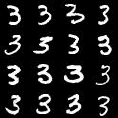
\includegraphics[width=0.21\textwidth]{figs/Fig_mnist_pairs_warmstart.png}%
\hspace{0.02\textwidth}%
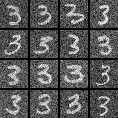
\includegraphics[width=0.21\textwidth]{figs/Fig_mnist_pairs_sa.png}%
\hspace{0.02\textwidth}%
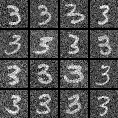
\includegraphics[width=0.21\textwidth]{figs/Fig_mnist_pairs_mala.png}

\small
\makebox[0.21\textwidth]{\centering (a) Warm-start (stored ``3'')}%
\hspace{0.02\textwidth}%
\makebox[0.21\textwidth]{\centering (b) SA endpoint}%
\hspace{0.02\textwidth}%
\makebox[0.21\textwidth]{\centering (c) MALA endpoint}
\caption{Paired before/after grids on MNIST digit ``3'' at $\beta{=}2000$. \textbf{Each cell is one independent chain; cell $(i,j)$ in panels (a, b, c) all share the same warm-start and the same seed.} Compare cell-by-cell \emph{across} panels, not within a row. (a) Stored ``3'' used as the warm-start. (b) SA chain endpoint after $T{=}5{,}000$ Langevin steps from that warm-start; digit identity is preserved while the textured background is the diffusive perturbation producing novelty (cf.\ Table~\ref{tab:mnist-baselines}). (c) MALA endpoint from the same warm-start and seed; visually identical to (b), so the Metropolis correction is unnecessary at $\alpha{=}0.01$. Bootstrap/Gaussian/Convex have no warm-start interpretation; see Table~\ref{tab:mnist-baselines} for numerical comparison.}
\label{fig:mnist-baselines}
\end{figure}

Each non-Langevin baseline failed on at least one axis (Table~\ref{tab:mnist-baselines}, Fig.~\ref{fig:mnist-baselines}): bootstrap by construction ($\mathcal{N}{=}0$), Gaussian perturbation by negligible noise, and random convex combination by mode collapse ($\bar{\mathcal{D}}{=}0.008$). DDPM failed entirely, producing samples indistinguishable from isotropic noise (max-$\cos{=}0.062$); a scaling study across $K\in\{100,\dots,3{,}500\}$ confirmed this failure persisted at all memory sizes tested (Appendix~\ref{app:scaling}). The VAE was the strongest learned baseline ($\mathcal{N}{=}0.214$, $\bar{\mathcal{D}}{=}0.441$). At $\beta{=}200$ (generation regime), SA dominated on both metrics: novelty $0.548$ ($2.6{\times}$ VAE), diversity $0.885$ ($2.0{\times}$ VAE). MALA's $99.2\%$ acceptance rate at $\alpha{=}0.01$ confirmed negligible ULA bias; a step-size sweep showed divergence only at $\alpha{\gtrsim}0.1$ (Appendix~\ref{app:stepsize-sweep}). The high-novelty $\beta{=}200$ samples reflected structured generation rather than high-temperature noise: a matched Gaussian control retained only $33\%$ cosine similarity to the nearest stored pattern vs.\ $45\%$ for SA (Appendix~\ref{app:noise-control}), and basin-crossing was genuine at $\beta{=}200$, where single-chain diversity ($0.796$) exceeded the multi-chain $\beta{=}2000$ value (Appendix~\ref{app:single-chain}). The advantage over the VAE was not an artifact of limited training data either: VAEs trained on $10{\times}$ and $100{\times}$ more images both fell short of SA on max-cosine similarity ($0.830$ vs.\ $0.848$) and diversity ($0.325$ vs.\ $0.600$) (Appendix~\ref{app:full-mnist-vae}). The SNR transition band (Proposition~\ref{prop:entropy-derivative}) thus delimited two regimes in the same algorithm: \emph{structured retrieval} ($\beta{=}2000$) and \emph{genuine generation} ($\beta{=}200$).

% ---------- Experiment 5: Protein Sequence Generation ----------
\paragraph{Protein sequence generation.}
We applied SA to protein sequences from the Pfam RNA Recognition Motif (RRM) family~\cite{mistryPfamProteinFamilies2021} (PF00076): $K{=}68$ aligned sequences, $L{=}71$ positions, one-hot encoded ($\mathbb{R}^{1420}$), PCA-reduced to $d{=}59$ (95\% variance retained), and $\ell_2$-normalized; the inverse PCA followed by per-position $\arg\max$ decoded chain endpoints back to amino acid sequences. This family size is typical of the low-data regime in which most Pfam families reside~\cite{finnPfamProteinFamilies2008}. The entropy inflection yielded $\beta^*{=}3.85$, half the random-pattern prediction $\sqrt{d}{=}7.68$, because conserved residues increase the effective similarity variance. We ran SA at $\beta{=}77$ ($20\beta^*$, retrieval) and $\beta{=}8$ ($2\beta^*$, generation) with the same 30-chain protocol.

\begin{table}[t]
\centering
\caption{Protein sequence generation on Pfam PF00076 ($K{=}68$, $d{=}59$). KL: global amino acid composition divergence. Pos-KL: mean per-position KL. MI~$r$: Pearson correlation of pairwise mutual information matrices. HMM: fraction passing the Pfam RRM hidden Markov model (HMM) at $E$-value~$<0.01$.}
\label{tab:protein-main}
\small
\begin{tabular}{@{}lcccccc@{}}
\toprule
Method & $\mathcal{N}$ $\uparrow$ & SeqID & KL $\downarrow$ & Pos-KL $\downarrow$ & MI~$r$ $\uparrow$ & HMM $\uparrow$ \\
\midrule
Bootstrap (replay)                  & $0.000$ & $0.644$ & $0.143$ & $7.52$ & $0.692$ & $100\%$ \\
VAE (latent${=}8$)                  & $0.621$ & $0.532$ & $0.416$ & $9.99$ & $0.525$ & $100\%$ \\
SA ($\beta{=}77$, retrieval)        & $0.243$ & $0.616$ & $0.107$ & $5.66$ & $0.733$ & $100\%$ \\
\textbf{SA ($\beta{=}8$, generation)} & $\mathbf{0.623}$ & $0.538$ & $\mathbf{0.060}$ & $\mathbf{2.92}$ & $\mathbf{0.871}$ & $100\%$ \\
\bottomrule
\end{tabular}
\end{table}

At generation temperature, SA matched the VAE on novelty ($0.623$ vs.\ $0.621$) while achieving $6.9{\times}$ lower amino acid composition divergence (KL$=0.060$ vs.\ $0.416$), $3.4{\times}$ lower per-position KL ($2.92$ vs.\ $9.99$), and $66\%$ higher co-evolutionary coupling fidelity (MI $r{=}0.871$ vs.\ $0.525$). The per-position metric is important because global composition KL alone cannot distinguish a method that preserves the correct amino acid at each position from one that merely matches overall frequencies; the $3.4{\times}$ gap confirmed that SA preserved position-specific conservation patterns that the VAE lost. All generated sequences passed the Pfam RRM HMM at $E$-value~$<0.01$ (HMMER~3.4~\cite{hmmer3}; median $8.1{\times}10^{-34}$), confirming that generated sequences were unambiguously recognized as RRM family members by an independent domain classifier. MALA at both temperatures produced near-identical results (acceptance $99.8\%$; $\Delta\mathrm{KL}<0.002$; Appendix~\ref{app:mala-generation}). Full results including all baselines and the per-position analysis are in Appendix~\ref{app:protein}. Because the Langevin gradient $\beta(\mathbf{T}(\boldsymbol{\xi})-\boldsymbol{\xi})$ is derived from the stored patterns at every step, stochastic attention preserved family-level structure at both position-specific and pairwise coupling levels even as samples explored far from individual sequences, while the VAE, which must learn the distribution from $K{=}68$ examples, could not maintain this fidelity when generating novel sequences. The temperature knob traded sequence identity for novelty ($0.243\to 0.623$) while \emph{improving} compositional fidelity (KL: $0.107\to 0.060$), a counterintuitive result explained by the fact that at lower $\beta$ the attention distribution spreads across more memories, producing samples that better reflect the family consensus rather than individual sequence idiosyncrasies. The observation that $\beta^*{=}3.85$ is half the random-pattern prediction $\sqrt{d}{=}7.68$ also has biological meaning: conserved residues in the RRM motif increase the effective variance of query-key similarities, shifting the phase boundary to lower temperature. Concurrent work~\cite{varnerTrainingFreeProtein2026} extends this pipeline to eight Pfam families and validates generated sequences structurally via ESMFold and AlphaFold2, finding that SA-generated sequences fold more accurately to canonical family structures than natural members in six of eight families tested. Additional MNIST digits and S\&P~500 log-returns at $d{=}424$ replicated the same ranking (Appendices~\ref{app:multidigit},~\ref{app:finance}); Olivetti faces at $d{=}4{,}096$ are covered next.

% ---------- Conditional generation via attention masking ----------
\paragraph{Conditional generation by masking the attention softmax.}
The masked update of Eq.~\eqref{eq:masked-sa} costs nothing beyond the unmasked sampler yet enables zero-shot subject-conditional generation. We applied SA to the Olivetti faces dataset (10 subjects, 10 portraits each, $K{=}100$, $d{=}4{,}096$, $\ell_2$-normalized; Appendix~\ref{app:olivetti}), which provides ground-truth subject labels for direct conditioning measurement. Without a mask, samples warm-started uniformly across all subjects and run at $\beta_{\mathrm{chain}}{=}200$ followed by a sharp readout at $\beta_{\mathrm{read}}{=}10{,}000$ landed on the target subject only $10.4\%$ of the time, indistinguishable from the random-guess rate of $10.0\%$. Setting $b_{k}{=}-\infty$ for memories outside a chosen subject lifted the same procedure to $96.0\%$ subject recovery, a $9.2{\times}$ improvement (Fig.~\ref{fig:olivetti}), with no learned classifier and no retraining. Conventional class-conditional generation requires either a classifier-guidance term added to the score function~\cite{songScoreBasedGenerativeModeling2021} or class-labeled training; the mask achieves the same effect with one Boolean vector and no learned components. The mask is the same Boolean operation used for causal attention in transformers, here applied along the memory axis rather than the sequence axis.

\begin{figure}[!t]
\centering
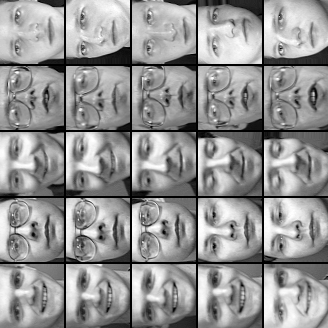
\includegraphics[width=0.235\textwidth]{figs/Fig_olivetti_stored.png}%
\hspace{0.01\textwidth}%
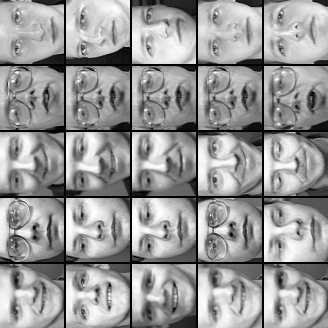
\includegraphics[width=0.235\textwidth]{figs/Fig_olivetti_masked.png}%
\hspace{0.01\textwidth}%
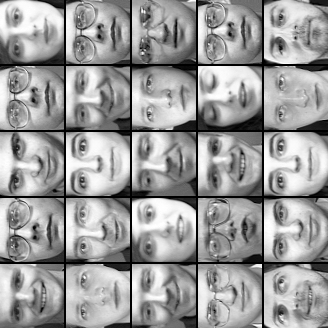
\includegraphics[width=0.235\textwidth]{figs/Fig_olivetti_unconditional.png}

\small
\makebox[0.235\textwidth]{\centering (a) Stored memories}%
\hspace{0.01\textwidth}%
\makebox[0.235\textwidth]{\centering (b) Hard-masked SA}%
\hspace{0.01\textwidth}%
\makebox[0.235\textwidth]{\centering (c) Unconditional SA}
\caption{Paired before/after grids on Olivetti faces ($K{=}100$, $d{=}4{,}096$). \textbf{Cell $(i,j)$ in all three panels uses the same warm-start: the $j$-th stored portrait of subject $i$.} (a) The 25 stored portraits used as warm-starts. (b) Hard-masked SA endpoints ($b_{k}{=}-\infty$ outside the row's subject); each row stays inside its subject (compare cell-by-cell to (a)). (c) Unconditional SA endpoints from the SAME warm-starts, mask removed; chains drift to other subjects within a row. Hard-mask subject-recovery: $96.0\%$ vs.\ unconditional $10.4\%$ vs.\ random-guess $10.0\%$.}
\label{fig:olivetti}
\end{figure}
